\documentclass{article}
\usepackage[spanish]{babel}
\usepackage[a4paper,top=2.54cm,bottom=2.54cm,left=2.54cm,right=2.54cm,marginparwidth=1.75cm]{geometry}
\usepackage{amsmath}
\usepackage{graphicx}
\usepackage{listings}
\usepackage{pgfplots}
\usepackage{xcolor}
\usepackage{pgf-pie}
\usepackage{enumitem}
\usepackage{listings}
\definecolor{python_color}{RGB}{255, 99, 71} % Color naranja para Python
\definecolor{cpp_color}{RGB}{65, 105, 225}   % Color azul para C++

\definecolor{pastelblue}{RGB}{102, 153, 204}
\definecolor{pastelred}{RGB}{255, 153, 153}
\definecolor{pastelgreen}{RGB}{102, 204, 102}
\definecolor{pastelyellow}{RGB}{255, 255, 153}
\definecolor{pastelpurple}{RGB}{153, 102, 204}
\definecolor{pastelteal}{RGB}{102, 204, 204}
\definecolor{pastelorange}{RGB}{255, 178, 102}
\definecolor{pastelgray}{RGB}{192, 192, 192}
\definecolor{pastellilac}{RGB}{204, 153, 255}
\definecolor{pastelpink}{RGB}{255, 153, 204}
\definecolor{pastellightblue}{RGB}{153, 204, 255}
\definecolor{pastelgold}{RGB}{255, 204, 153}
\definecolor{mician}{RGB}{0, 120, 135}
\definecolor{fucsia}{RGB}{176, 87, 141}
\definecolor{verdeoscuro}{RGB}{0, 100, 0}
\pgfplotsset{compat=1.17}
\lstset{
    language=Python,
    basicstyle=\ttfamily,
    keywordstyle=\color{fucsia},
    commentstyle=\color{verdeoscuro},
    numbers=left,
    numberstyle=\tiny,
    numbersep=5pt,
    breaklines=true,
    frame=single
}

\begin{document}
    \begin{titlepage}
        \centering
        \vspace*{0.5cm}
        \vspace{1cm}
        
\includegraphics[width=0.4\textwidth]{utdt-logo.jpg} \\
        \vspace{1cm}
        \Large{\bfseries{TD V: Diseño de Algoritmos}}\\
        \vspace{0.8cm}
        \Large{Trabajo Práctico 1}\\
        \vspace{0.5cm}
        \text{Primer Cuatrimestre del 2024} \\
        \vspace{6cm}
        
        \Large{Autores:}\\
        \vspace{0.5cm}
        \Large{Aufiero, Catalina}\\
        \vspace{0.2cm}
        \Large{Brusco, Catalina}\\
        \vspace{0.2cm}
        \Large{Castore, Juan Ignacio}\\

        
        \vfill
        
        \large{Abril del 2024}
    \end{titlepage} 

\section{Introducción}
    \vspace{0.5cm}
    La aproximación de datos mediante funciones es una herramienta fundamental en diversas disciplinas científicas y tecnológicas. Permite modelar de manera eficiente fenómenos complejos que exhiben comportamientos diversos y a menudo intrincados. La tarea de aproximar datos se vuelve desafiante cuando estos provienen de funciones desconocidas con comportamientos no lineales y variaciones bruscas. En tales casos, encontrar una representación funcional adecuada puede ser crucial para comprender y predecir el comportamiento del fenómeno en cuestión. Aquí es donde entran en juego las funciones lineales continuas a trozos (PWL). Se define como Piecewise Linear a toda función continua definida en intervalos o segmentos, donde cada segmento es una línea recta; siendo entonces múltiples tramos de líneas rectas conectados entre sí en determinados puntos llamados "breakpoints".

    El problema central que se abordará en este trabajo es el de encontrar una función continua PWL que aproxime de manera óptima un conjunto de puntos dados. Esta función debe ser capaz de capturar las características principales de los datos y minimizar el error de aproximación. Para ello, se diseñarán y evaluarán varios algoritmos con diferentes enfoques y estrategias de optimización.

    El objetivo principal de este trabajo es desarrollar métodos efectivos y eficientes para la aproximación de datos mediante funciones PWL. Esto incluye el diseño de algoritmos que sean capaces de manejar conjuntos de datos grandes y complejos, así como la evaluación de su rendimiento y calidad en una variedad de escenarios y situaciones prácticas.
    
    Se implementará el modelo con tres algoritmos -Fuerza Bruta, Backtracking y Programación Dinámica- en Pyhton y C++. A continuación, se detallará el proceso de desarrollo de cada algoritmo, incluyendo su experimentación con diversas instancias, las diferencias entre ellos y su rendimiento en términos de eficiencia y precisión. El objetivo principal es realizar una comparación exhaustiva de estas implementaciones, proporcionando una visión clara y detallada de cómo estas herramientas pueden ser útiles en la predicción de fenómenos.
    
    \\
 
\section{Modelo}
    \vspace{0.5cm}
    Para resolver este problema, se generará una variedad de funciones PWL (Piecewise Linear), con el objetivo de encontrar aquella que minimice el error dada una grilla y una instancia de datos. El proceso de aproximación consta de varias etapas. En primer lugar, se construye una grilla que define el dominio de la función y proporciona los puntos de referencia para la aproximación. Luego, se discretizan los datos observados de manera homogénea, lo que nos permite trabajar con ellos de manera más efectiva. A continuación, se ajusta una función PWL a estos datos, dividiendo el dominio en segmentos y aproximando los datos dentro de cada segmento con una función lineal.
    \\
    
\section{Algoritmos}
    \vspace{0.5cm}
    \subsection{Fuerza Bruta}
        El método de Fuerza Bruta consiste en generar todas las posibles soluciones para un problema, explorando exhaustivamente todas las combinaciones desde el primer dato observado hasta el último. Esta implementación se realiza de manera recursiva, buscando todas las combinaciones de soluciones viables. Dada una grilla y una cantidad de segmentos determinada, se consideran soluciones factibles aquellas que cumplen cuatro condiciones:
        \begin{enumerate}
            \item Comienzan desde la primera discretización de la grilla del eje $x$ y terminan en la última discretización del eje $x$.
            \item La función lineal resultante es continua, lo que significa que cada breakpoint se encuentra de manera consecutiva, sin interrupciones.
            \item La función lineal resultante es inyectiva, los breakpoints no pueden repetir valores en el eje x.
            \item Son soluciones completas, es decir, tienen la cantidad de segmentos+1. 
        \end{enumerate}
        
        Durante su ejecución, el algoritmo siempre compara la mejor solución factible encontrada hasta el momento, es decir, aquella que tenga el menor error, con otras soluciones factibles.  

        Este enfoque, sencillo de implementar, resulta ser computacionalmente costoso, ya que explora todas las opciones sin utilizar ninguna poda de factibilidad ni optimalidad en las soluciones parciales. Sin embargo, en ciertos casos donde el espacio de búsqueda es pequeño o no existe una solución más eficiente conocida, el método de Fuerza Bruta puede ser una opción viable.

        \subsubsection{Pseudocódigo}
        
        \begin{lstlisting}[language=pseudocode]
FuerzaBruta(best, actual, grid_x, grid_y, instance)

  si |actual| == |best| y actual es factible:
    Calculo el error
    si el error es < error de best:
      Actualizo best
      retorno (caso base)

  si |actual| == |best|:
    retorno (llegue a una solucion posible, pero no factible)

  si no:
    para j en rango(grid_x):
      para i en rango(grid_y):
        Agrego (i,j) en actual
        FuerzaBruta(best, actual, grid_x, grid_y, instance)
        Saco (i,j) de actual
\end{lstlisting}


        \subsubsection{Implementación en Python}
        El problema se materializa en una grilla, lo que requirió la implementación de la clase Punto. Esta clase encapsula las coordenadas de los breakpoints dentro de la grilla, lo que facilita el cálculo del error de los datos observados y la distancia a la recta.

        La implementación en Python utiliza un enfoque basado en un diccionario para representar la mejor solución encontrada hasta el momento. Este diccionario contiene: la cantidad de breakpoints, la mejor solucion encontrada hasta el momento -de tipo lista con las posiciones de los breakpoints de la PWL-;  y su mínimo error. Esta representación ofrece la ventaja de permitir una actualización fácil de la mejor solución a medida que avanza el algoritmo, y a su vez a medida que generamos posibles soluciones. 
        
        Una ventaja significativa, es su facilidad de uso y flexibilidad gracias a las características dinámicas del lenguaje, como las listas dinámicas y la capacidad de trabajar con diccionarios de manera intuitiva. Esto facilita el desarrollo y la depuración del código.

        Sin embargo, esta implementación puede tener una desventaja en términos de eficiencia computacional, especialmente en conjuntos de datos grandes. La necesidad de realizar copias de las soluciones para evitar modificaciones accidentales puede generar un costo adicional en términos de memoria y tiempo de ejecución, especialmente cuando se trata de conjuntos de datos muy grandes. 

        \subsubsection{Implementación en C++}

        
        La implementación en C++ requirió la definición de varias clases adicionales, además de Punto. Entre ellas se encuentran Solución Posible, Mejor Solución o Best y Grilla. La clase Solución Posible se encarga de representar las soluciones parciales (como vectores de Puntos), incorporando funciones para verificar la factibilidad y calcular el error cuando es una solucion completa. Por otro lado, Mejor Solución almacena la mejor solución encontrada durante la ejecución del algoritmo, así como su error mínimo. Por último, Grilla proporciona la estructura necesaria para definir la disposición de los puntos, los cuales generan soluciones candidatas y son esenciales para evaluar el error de aproximación en comparación con los puntos observados.
        
        Esta implementación en C++ implica una arquitectura más robusta y estructurada que la anterior. A su vez, a diferencia de Python, C++ utiliza arreglos estáticos con un tamaño predefinido debido a su naturaleza de memoria estática; y tiene mejor manejo de memoria ya que evita realizar copias innecesarias de ciertos datos grandes, como la grilla, tomándolos como referencia.
        

    \subsection{Backtracking}
    Backtracking es otra técnica de búsqueda exhaustiva para encontrar soluciones que explora todas las opciones disponibles y retrocede cuando se encuentra una solución que no cumple con ciertas condiciones. Para reducir las soluciones posibles, se implementan podas de factibilidad (las mismas que en Fuerza Bruta) y optimalidad, esto último mejora la eficiencia del algoritmo en comparación con el anterior. El algoritmo recursivo deja de explorar aquellas soluciones donde:
    
    \begin{enumerate}
            \item El error acumulado de la solución parcial ya es mayor que el mínimo error encontrado hasta el momento. (Poda por optimalidad)
            \item La solución parcial no tiene el primer breakpoint en la primera discretización de la grilla del eje $x$ ni termina en la última discretización del eje $x$. (Poda por factibilidad)
            \item La solución parcial no es inyectiva.(Poda por factibilidad)
        \end{enumerate}
    
   Estas técnicas de poda permiten reducir el espacio de búsqueda y mejorar significativamente la eficiencia del algoritmo de backtracking en comparación con Fuerza Bruta. 
   	
   	\subsubsection{Pseudocódigo}
   	
   	\begin{lstlisting}[language=pseudocode]
BackTracking(best, actual, grid_x, grid_y, instance)

  si |actual| == |best| y actual es factible:
    Calculo el error
    si el error es < error de best:
      Actualizo best
      retorno (caso base)

  si |actual| == |best| o actual no es funcion:
    (poda por factibilidad)
    retorno

  si |actual| > 1 y error actual > error de best:
    (poda por optimalidad)
    retorno (error actual > best error con al menos 2 breakpoints)

  si no:
    para j en rango(grid_x):
      para i en rango(grid_y):
        Agrego (i,j) en actual
        BackTracking(best, actual, grid_x, grid_y, instance)
        Saco (i,j) de actual
\end{lstlisting}
	
   	
        \subsubsection{Implementación en Python}
        
        La implementación en Python utiliza el algoritmo de Fuerza Bruta y ajusta por el uso de las podas ciertas funciones. A diferencia de F.B., es necesario: implementar la función EsFuncion que admiten soluciones parciales y verifican su factibilidad; modificar la función Error que admite tanto soluciones parciales como aquellas completas para calcular el error acumulado; y empleando las podas anteriores, integrarlo a la función recursiva.
        
        
       
        Mientras que en el enfoque de Fuerza Bruta se generan todas las posibles soluciones antes de buscar la mejor; en BackTracking, se generan solamente aquellas posibles soluciones y mejores que la encontrada hasta el momento.  
        
         
        \subsubsection{Implementación en C++}
       Dicha implementación emplea las mismas podas (implementadas en VaSerFactible y esFuncion) que en Python y también resulta ser una extensión modificada del enfoque de Fuerza Bruta. 
       
    

        \subsection{Programación  Dinámica}
        
        Programación Dinámica es una técnica que permite construir una solución óptima a partir de subproblemas más pequeños. El algoritmo para resolver el problema utiliza una matriz tridimensional. Cada dimensión de esta matriz representa la cantidad de breakpoints utilizados en la solución. Además, cada nivel de la matriz está asociado a una matriz del tamaño de la grilla, donde se almacenan múltiples soluciones potenciales, pero solo una de ellas presenta el error mínimo.
        

        
        En primer lugar, se genera y calcula la matriz para el nivel uno, donde se asume que la función PWL tiene dos breakpoints. Esta matriz determina el error mínimo desde el primer eje hasta el último eje x. Si la instancia del problema implica más de dos breakpoints, las matrices para los niveles posteriores se construirán utilizando el mínimo error encontrado en el nivel anterior.
        

        
        Para reconstruir el camino, tambien se contruye una matriz que a partir del minimo error del ultimo eje x, decide el punto del eje x anterior. Lo anterior se repite hasta llegar al primer punto en el eje x. Consecuentemente, para encontrar el camino con error minimo retrocede desde el último punto hasta el primero, siguiendo la ruta con el menor error acumulado.


\subsubsection{Pseudocódigo}
        

        \begin{lstlisting}[language=pseudocode]
ProgramDinam(best, cantSegmentos, grid_x, grid_y, instance)

  para j entre 1 y cantSegmentos:
    Creamos matriz_nivel[x][y] y matriz_vuelta[x][y]

    si es la primera iteración:
      res = ProgramDinamK1()  # ¿Llamamos a la funcion que llena la matriz con 1 segmento?
    si no:
      res = ProgramDinamKN()  # ¿Llamamos a la funcion que llena la matriz con j segmentos?

    Guarda la matriz_nivel y la matriz_vuelta
    Buscamos el error minimo en la ultima matriz nivel
    Reconstruimos la solucion usando la matriz vuelta
\end{lstlisting}

        
         
\subsubsection{Implementación en Python}
            La idea del algortimo implementado es ir rellenando una matriz por una cantidad especifica de segmentos, e ir usando esas matrices para calcular otras matrices. En otras palabras, la idea es primero hacer una matriz para cuando hay 1 segmento, y rellenar esta con todos los valores correspondientes. Esto se lleva a cabo en la función ProgramDinamK1, calculando los errores desde cada coordenada (x,y), salvo las de la primera columna, hasta todos los puntos de la primera columna.
            
            Luego de calcular la matriz con cantidadSegmentos = 1, tenemos otra función (ProgramDinamKN) donde calculamos los errores de toda la matriz para cantSegmentos = N, donde usamos la matriz de cantSegmentos = N-1. La idea sería calcular el error desde cada punto (i,j) que este entre la columna numero cantSegmentos+1 (suponiendo que la primera columna es la columna 0) y la última columna, hasta todos los puntos que estén entre la columna número cantSegmentos y la columna j. Luego de encontrar este error, se le suma el error que esta guardado en la matriz[cantSegmentos-2], que sería la matriz " anterior" que tiene los errores cuando hay 1 segmento menos, y esta suma se guarda en la nueva matriz. Esto esta dentro de un for que va desde 1 hasta la cantidad de segmentos totales, y dónde la última matriz, en la última columna estarán los errores finales, y entre ellos el error mínimo que devolvería la PWL.

            Por último, para luego poder reconstruir la respuesta, lo que hicimos fue tener una matriz alternativa donde guardamos en vez de los errores minimos, la coordenada que generaba ese error minimo. Entonces, para reconstruirla, tomamos la ultima matriz[x][y] de errores, nos fijamos en la última columna el error mínimo y agregamos esa coordenada al vector respuesta, ya que esta iba a ser la última coordenada de la solución. Luego fuimos a la matriz-vuelta, que es la que contiene las coordenadas, a la última matriz (matriz[cantSegmentos-1]), y buscamos qué coordeanda estaba guardada en la posición que ya guardamos en el vector respuesta. Luego agregamos esta coordenada al vector respuesta, y fuimos a la matriz[cantSegmentos-2] a buscar en esa posición, la próxima coordenada. Y así sucesivamente hasta llegar a la matriz-vuelta[0] que contendrá la primera coordenada. En el vector respuesta tendremos el camino que hace PWL.
            
            Para realizar esto usamos una lista de lista de listas, es decir, matriz[k][x][y], siendo k=cantidad de segmentos, las Xs y las Ys.
            El pseudocódigo de este algortimo es el siguiente:
            

            
            \subsubsection{Implementación en C++}
            En C++, implementamos el mismo algoritmo que en python, pero tuvimos que hacer algunos cambios ya que las estructuras en cada lenguaje cambian. Hicimos la matriz de tres dimensiones como vector de un vector de vectores. Usamos dos de estas matrices de tres dimensiones al igual que en python, una para guardar los errores y otra para guardar las coordenadas.

            Otra cosa que podemos destacar de C++, es que el mismo algoritmo implementado en Python y en C++ genera una diferencia en el tiempo de ejecución. Es soprendente la diferencia de tiempos que esta tiene, al ser C++ mucho más rápido, lo que se debe a que Python es un lenguaje interpretado mientras que C++ es un lenguaje compilado.

\section{Experimentación}
\vspace{0.5cm}
        A la hora de decidir el tamaño de la grilla y la cantidad de segmentos, surge un balance entre la minimización del error y el incremento en el tiempo de ejecución de los algoritmos. Por ende, es recomendable seleccionar una configuración de grilla y segmentos que reduzca el error de manera efectiva, al mismo tiempo que mantenga una ejecución razonable en términos de tiempo, en los diferentes algoritmos.

        En las siguientes figuras se muestra la mejor solución de cada instancia dado una grilla de 6x6 y 4 segmentos. Se puede observar como la discretización se ajusta a la instancia (los datos observados) y la PWL que minimiza el error.

    \begin{figure}[h!]
          \centering
          \begin{minipage}{.3\textwidth}
            \centering
            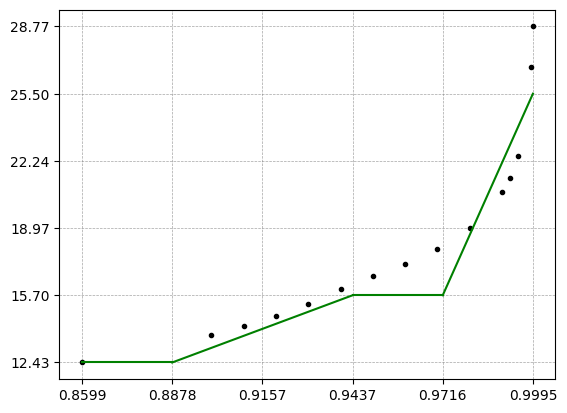
\includegraphics[width=.8\linewidth]{graficos/aspen_6x6_4.png}
            \caption{Instancia Aspen}
          \end{minipage}%
          \begin{minipage}{.3\textwidth}
            \centering
            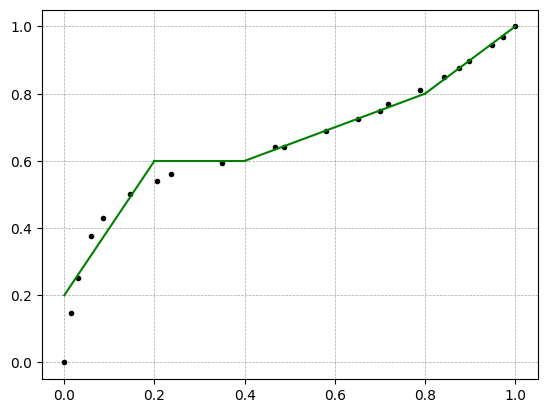
\includegraphics[width=.8\linewidth]{graficos/ethanol_6x6_4.png}
            \caption{Instancia Ethanol}
          \end{minipage}%
          \begin{minipage}{.3\textwidth}
            \centering
            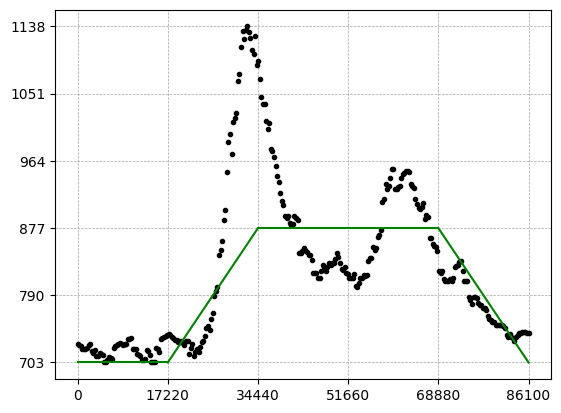
\includegraphics[width=.8\linewidth]{graficos/optimistic_6x6_4.png}
            \caption{Instancia Optimistic}
          \end{minipage}%
          
    \end{figure}
    
    \begin{figure}[h!]
          \centering
            \begin{minipage}{.3\textwidth}
            \centering
            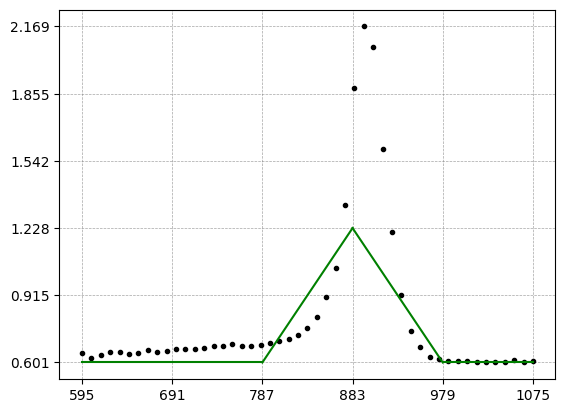
\includegraphics[width=.8\linewidth]{graficos/titanium_6x6_4.png}
            \caption{Instancia Titanium}
          \end{minipage}%
          \begin{minipage}{.3\textwidth}
            \centering
            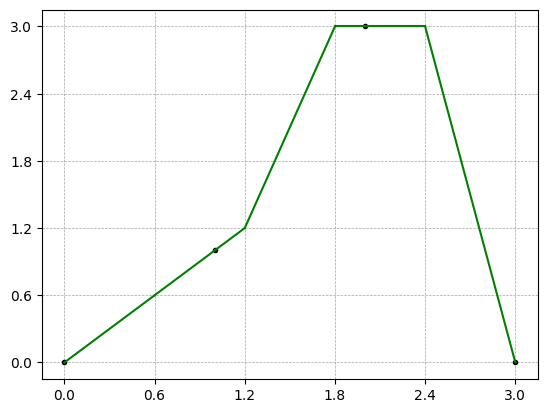
\includegraphics[width=.8\linewidth]{graficos/toy_6x6_4.png}
            \caption{Instancia Toy}
          \end{minipage}%
        \end{figure}
    \subsubsection{Tiempo de ejecución según el algoritmo}
    Para analizar los tiempos de ejecución de los distintos algoritmos, exploramos las instancias Titanium y Aspen. A priori intuíamos que los algoritmos implementados en C++, demorarían menos debido a la naturaleza compilada del lenguaje y por el uso de referencia al mandar los parámetros. En el Cuadro 1, se muestra el tiempo en segundos que cada algoritmo requirió para completar su ejecución, llegando a la misma solución y error mínimo. 
    
    Como era de esperar, Fuerza Bruta fue el algoritmo más lento debido a su enfoque, generar todas las posibles soluciones para resolver el problema.

    En segundo lugar en términos de tiempo de ejecución, encontramos Backtracking. Aquí, la versión en C++ superó en velocidad a la implementación en Python, completando la tarea cuatro veces más rápido.A su vez, como ya hemos comentado antes, la diferencia de dicho algoritmo con Fuerza Bruta es la implementación de podas, como podemos observar en el gráfico mejora en más de la mitad los tiempos. 

    Finalmente, Programación Dinámica demostró ser el enfoque más eficiente, siendo considerablemente más rápido que los otros algoritmos. Esta diferencia en rendimiento podría atribuirse a la capacidad de Programación Dinámica para almacenar información previamente calculada, evitando así la repetición de cálculos. Este hallazgo resultó sorprendente ya que no teníamos una idea clara de cuál de los últimos dos algoritmos sería más rápido. En la instancia Titanium, encontramos que Programación Dinámica fue casi 3 veces más rápido en Python y aproximadamente 9 veces más rápido en C++ en comparación con BackTracking.
 

    En la instancia Aspen, como podemos observar en el Cuadro 1, obtuvimos resultados similares a los de la Instancia Titanium, utilizando la misma configuración de grilla y cantidad de breakpoints. Los tiempos de ejecución para cada algoritmo fueron prácticamente idénticos en ambas instancias. 

    Por lo tanto, descubrimos que la eficiencia del algoritmo varía significativamente según la técnica utilizada. Programación Dinámica ofrece mejoras de rendimiento significativas al minimizar la repetición de cálculos (siempre y cuando sea implementado en el mismo lenguaje). A su vez, es interesante notar las diferencias en el rendimiento según el lenguaje de programación; el tiempo demorado en Backtracking con C++ es menor que el de Programación Dinámica en Python.

    \begin{table}[htbp]
        \centering
        \caption{Tiempos de ejecución de los algoritmos (Grilla 6x6 con 4 breakpoints)}
        \begin{tabular}{|c|c|c|c|c|c|c|}
            \hline
            \text{Instancia} & \text{F.B. Python} & \text{F.B. C++} & \text{B.T. Python} & \text{B.T. C++} & \text{P.D. Python} & \text{P.D. C++} \\
            \hline
            Titanium & 75 & XX & 0.33 & 0.08 & 0.12 & 0.00916 \\
            Aspen & 67.76 & XX & 0.28 & 0.06 & 0.085 & 0.0017 \\
            \hline
        \end{tabular}
    \end{table}

    \subsubsection{Programación Dinámica implementada con múltiples k y misma grilla}
    Para entender la importancia de implementar diferentes breakpoints en la solución del problema, decidimos explorar la instancia Optimistic utilizando una grilla de 11x11 y aplicando el algoritmo de Programacion Dinamica implementado en python para analizar el mínimo error obtenido. Nuestra hipótesis inicial era que una mayor cantidad de breakpoints conduciría a un menor error, ya que permitiría una aproximación más precisa de los datos observados.

    Las Figuras 6 a 14 muestran los resultados obtenidos al variar la cantidad de segmentos (k) en la grilla fija de 11x11. Como se puede observar, efectivamente, el error tiende a decrecer a medida que aumenta la cantidad de segmentos utilizados. Esto respalda nuestra intuición de que una mayor granularidad en la aproximación puede mejorar la precisión de la solución.

    Sin embargo, surge una observación interesante al analizar los resultados obtenidos con una mayor cantidad de segmentos. A partir de 7 segmentos en esta grilla de 11x11, el error comienza a incrementar nuevamente. Este hallazgo sugiere que agregar más segmentos no siempre conduce a una mejora en la precisión de la aproximación, especialmente cuando se alcanza un cierto punto de saturación. Nuestra hipótesis al respecto es que, a veces, al agregar demasiados segmentos en una grilla sin aumentar la discretización de esta, provoca que la PWL realice "saltos en zigzag" donde no los haría si tuviera menos segmentos que colocar.

    Estos resultados nos permiten entender cómo la elección de la cantidad de breakpoints puede afectar el rendimiento y la precisión de la aproximación. Además, sirve de guía acerca de cuál es la cantidad óptima de segmentos a utilizar en función de la discretización dada, resaltando la importancia de un análisis cuidadoso al diseñar algoritmos para resolver este tipo de problemas.                                                                                              

   
    
\begin{figure}[ht]
    \centering
    \begin{minipage}{.3\textwidth}
        \centering
        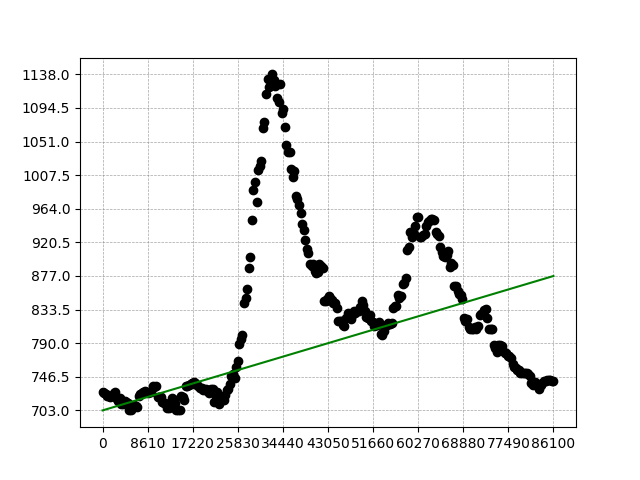
\includegraphics[width=.9\linewidth]{graficos/solution_11x11,1N_optimistic_instance.png}
        \caption{k=1, error = 21646}
    \end{minipage}%
    \begin{minipage}{.3\textwidth}
        \centering
        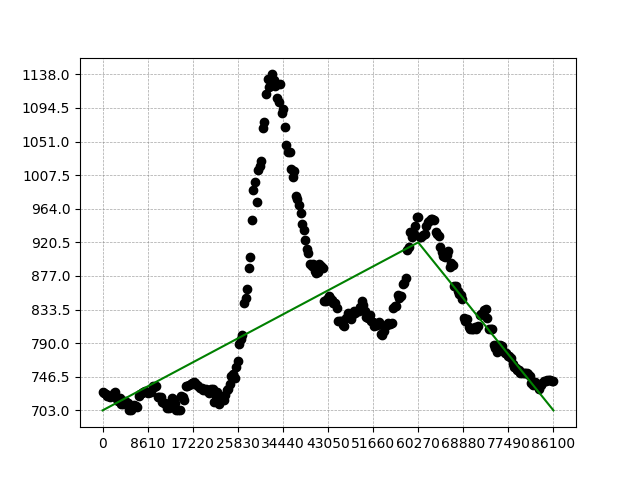
\includegraphics[width=.9\linewidth]{graficos/solution_11x11,2N_optimistic_instance.png}
        \caption{k=2, error = 15359}
    \end{minipage}%
    \begin{minipage}{.3\textwidth}
        \centering
        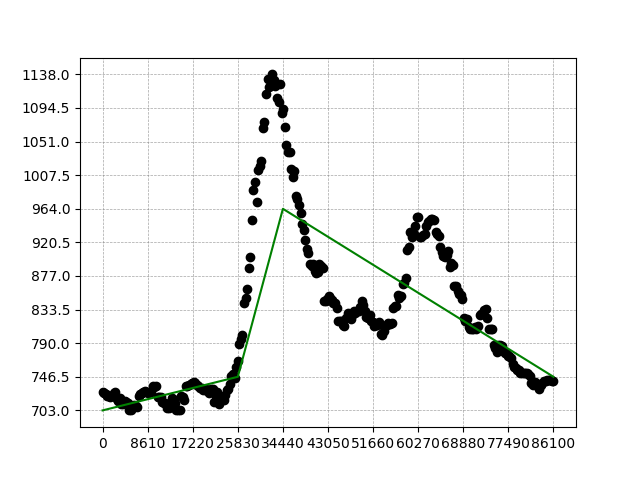
\includegraphics[width=.9\linewidth]{graficos/solution_11x11,3N_optimistic_instance.png}
        \caption{k=3, error = 13408}
    \end{minipage}%
\end{figure}

\begin{figure}[h!]
          \centering
          \begin{minipage}{.3\textwidth}
            \centering
            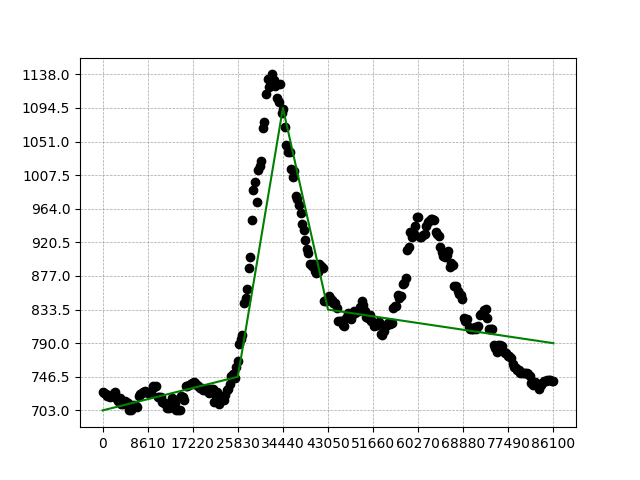
\includegraphics[width=.9\linewidth]{graficos/solution_11x11,4N_optimistic_instance.png}
            \caption{k=4, error = 10168 }
          \end{minipage}%
          \begin{minipage}{.3\textwidth}
            \centering
            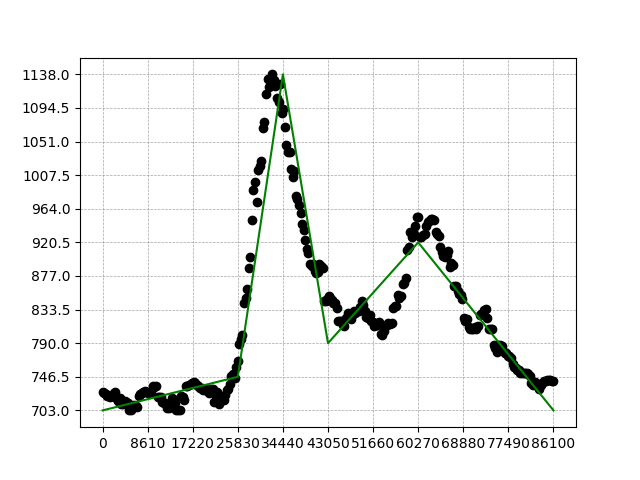
\includegraphics[width=.9\linewidth]{graficos/solution_11x11,5N_optimistic_instance.png}
            \caption{k=5, error = 7115 }
          \end{minipage}%
          \begin{minipage}{.3\textwidth}
            \centering
            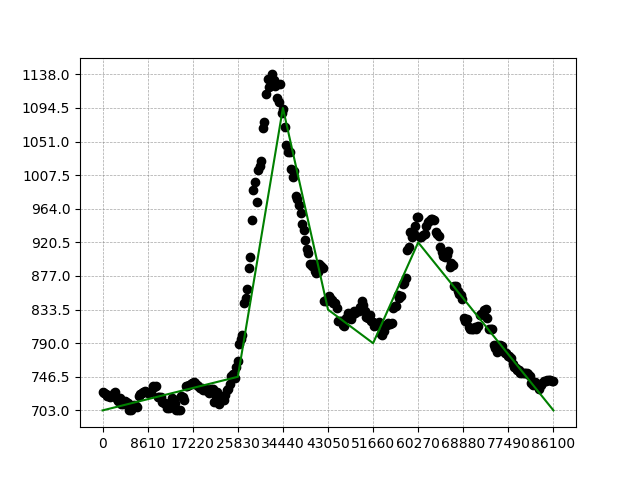
\includegraphics[width=.9\linewidth]{graficos/solution_11x11,6N_optimistic_instance.png}
            \caption{k=6, error = 6589}
          \end{minipage}%
          
    \end{figure}
    \begin{figure}[h!]
          \centering
          \begin{minipage}{.3\textwidth}
            \centering
            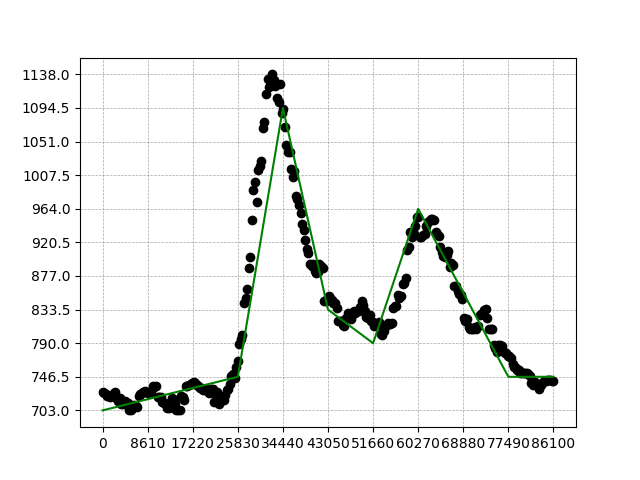
\includegraphics[width=.9\linewidth]{graficos/solution_11x11,7N_optimistic_instance.png}
            \caption{k=7, error = 6529}
          \end{minipage}%
          \begin{minipage}{.3\textwidth}
            \centering
            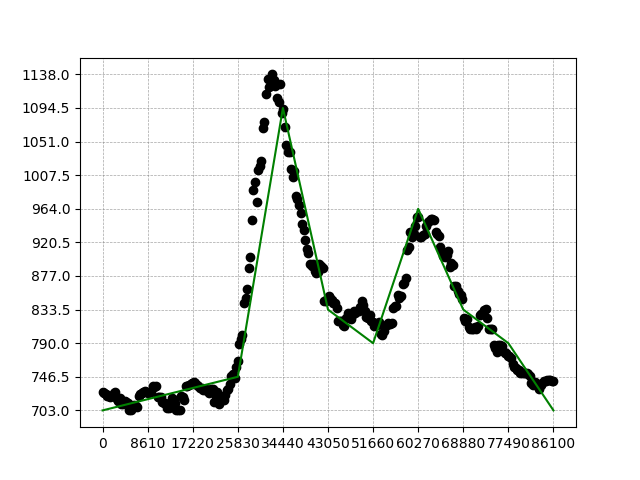
\includegraphics[width=.9\linewidth]{graficos/solution_11x11,8N_optimistic_instance.png}
            \caption{k=8, error = 6625}
          \end{minipage}%
          \begin{minipage}{.3\textwidth}
            \centering
            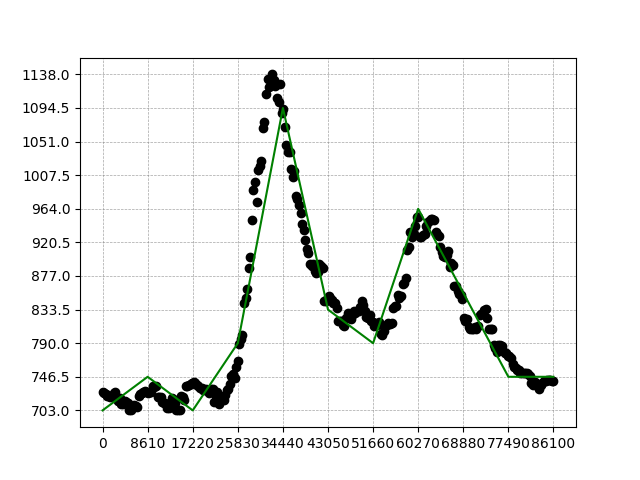
\includegraphics[width=.9\linewidth]{graficos/solution_11x11,9N_optimistic_instance.png}
            \caption{k=9, error = 6715}
          \end{minipage}%
    \end{figure}
    
\clearpage

\section{Conclusión}
    \vspace{0.5cm}

Para concluir, las funciones Piecewise Linear (PWL) son una herramienta esencial en disciplinas científicas y tecnológicas para aproximar diversos fenómenos. Pudimos modelar eficientemente fenómenos no lineales con tres algoritmos que tienen enfoques y estrategias diferentes para encontrar la solución óptima, con Programación Dinámica destacándose como el más eficiente. Su experimentación revela la importancia de la selección adecuada del tamaño de la grilla y la cantidad de segmentos en la aproximación de datos. Si bien agregar más segmentos puede mejorar la precisión, existe un punto de saturación donde el error comienza a aumentar nuevamente.

En futuras investigaciones sería interesante estudiar el impacto de diferentes configuraciones de grilla  y segmentos, empleando grillas no equidistantes/cuadradas porque podría haber una relacion entre la disretización y los datos. Lo anterior creemos que podría lograrse con métodos de discretización adaptativos que optimicen la distribución de los puntos en función de la complejidad de los datos.
    
\end{document}


CONSIGNA: 

 El modelo, la descripción de los algoritmos, los operadores, las decisiones de diseño, la
implementación, el testing realizado, la presentación de resultados, instrucciones de
compilación y ejecución.
La resolución
del trabajo se compone de varias etapas, incluyendo el diseño de 3 algoritmos, programación,
experimentación, así también como el reporte detallado de la evaluación de los métodos
implementados, los resultados obtenidos y la discusión sobre el caso real.
---------------------------------------------------------------------------------
